% ------------------------------------------------------------------------
% ------------------------------------------------------------------------
% abnTeX2: Modelo de Projeto de pesquisa em conformidade com 
% ABNT NBR 15287:2011 Informação e documentação - Projeto de pesquisa -
% Apresentação 
% ------------------------------------------------------------------------ 
% ------------------------------------------------------------------------

\documentclass[
	% -- opções da classe memoir --
	12pt,				% tamanho da fonte
	openright,			% capítulos começam em pág ímpar (insere página vazia caso preciso)
	twoside,			% para impressão em recto e verso. Oposto a oneside
	a4paper,			% tamanho do papel. 
	% -- opções da classe abntex2 --
	%chapter=TITLE,		% títulos de capítulos convertidos em letras maiúsculas
	%section=TITLE,		% títulos de seções convertidos em letras maiúsculas
	%subsection=TITLE,	% títulos de subseções convertidos em letras maiúsculas
	%subsubsection=TITLE,% títulos de subsubseções convertidos em letras maiúsculas
	% -- opções do pacote babel --
	english,			% idioma adicional para hifenização
	french,				% idioma adicional para hifenização
	spanish,			% idioma adicional para hifenização
	brazil,				% o último idioma é o principal do documento
	]{abntex2}

% ---
% PACOTES
% ---

% ---
% Pacotes fundamentais 
% ---
\usepackage{lmodern}			% Usa a fonte Latin Modern
\usepackage[T1]{fontenc}		% Selecao de codigos de fonte.
\usepackage[utf8]{inputenc}		% Codificacao do documento (conversão automática dos acentos)
\usepackage{indentfirst}		% Indenta o primeiro parágrafo de cada seção.
\usepackage{color}				% Controle das cores
\usepackage{graphicx}			% Inclusão de gráficos
\usepackage{microtype} 			% para melhorias de justificação
\usepackage[table,xcdraw]{xcolor}
\usepackage{amsmath}
\usepackage{lscape}
\usepackage{array}
\newcolumntype{L}[1]{>{\raggedright\let\newline\\\arraybackslash\hspace{0pt}}m{#1}}
\newcolumntype{C}[1]{>{\centering\let\newline\\\arraybackslash\hspace{0pt}}m{#1}}
\newcolumntype{R}[1]{>{\raggedleft\let\newline\\\arraybackslash\hspace{0pt}}m{#1}}

% ---

% ---
% Pacotes adicionais, usados apenas no âmbito do Modelo Canônico do abnteX2
% ---
%\usepackage{lipsum}				% para geração de dummy text
% ---

% ---
% Pacotes de citações
% ---
\usepackage[brazilian,hyperpageref]{backref}	 % Paginas com as citações na bibl
\usepackage[alf]{abntex2cite}	% Citações padrão ABNT

% --- 
% CONFIGURAÇÕES DE PACOTES
% --- 

% ---
% Configurações do pacote backref
% Usado sem a opção hyperpageref de backref
%\renewcommand{\backrefpagesname}{Cited on page:~}
% Texto padrão antes do número das páginas
\renewcommand{\backref}{Cited on page: }
% Define os textos da citação
%\renewcommand*{\backrefalt}[4]{
%	\ifcase #1 %
%		Nenhuma citação no texto.%
%	\or
%		Cited on page #2.%
%	\else
%		CiteCitado #1 vezes nas páginas #2.%
%	\fi}%
% ---

\addto\captionsbrazil{%
	\renewcommand{\listfigurename}{Figure list}
	\renewcommand{\figurename}{Fig.}
	\renewcommand{\tablename}{Table}
	\renewcommand{\listtablename}{Table list}
	\renewcommand{\contentsname}{Summary}
	\renewcommand{\bibname}{References}
%	\renewcommand{\abstract}{abstract}
%	\renewcommand{\abstract}[2]{\noindent\textbf{\textsl{\space#1---}#2}\\}
}
% ---
% Informações de dados para CAPA e FOLHA DE ROSTO
% ---
\titulo{Development and implementation and  of a coarse-grained Protein-DNA/RNA docking model}
\autor{Rodrigo Vargas Honorato}
\local{Brazil}
\data{2017}
\instituicao{%
  Centro Nacional de Pesquisa em Energia e Materiais - CNPEM
  \par
  Laboratório Nacional de Biociências - LNBio
  \par
  Laboratório de Biologia Computacional - LBC}
\tipotrabalho{Research project}
% O preambulo deve conter o tipo do trabalho, o objetivo, 
% o nome da instituição e a área de concentração 
\preambulo{Research project submission as requirement of FAPESP Research Fellowships Abroad (BPE) for scientists who have a permanent position in a research institution in the State of São Paulo and obtain a leave of absence to develop a research project in a foreign institution.}
% ---

% ---
% Configurações de aparência do PDF final

% alterando o aspecto da cor azul
\definecolor{blue}{RGB}{41,5,195}

% informações do PDF
\makeatletter
\hypersetup{
     	%pagebackref=true,
		pdftitle={\@title}, 
		pdfauthor={\@author},
    	pdfsubject={\imprimirpreambulo},
	    pdfcreator={LaTeX with abnTeX2},
		pdfkeywords={abnt}{latex}{abntex}{abntex2}{projeto de pesquisa}, 
		colorlinks=true,       		% false: boxed links; true: colored links
    	linkcolor=blue,          	% color of internal links
    	citecolor=blue,        		% color of links to bibliography
    	filecolor=magenta,      		% color of file links
		urlcolor=blue,
		bookmarksdepth=4
}
\makeatother
% --- 

% --- 
% Espaçamentos entre linhas e parágrafos 
% --- 

% O tamanho do parágrafo é dado por:
\setlength{\parindent}{1.3cm}

% Controle do espaçamento entre um parágrafo e outro:
\setlength{\parskip}{0.2cm}  % tente também \onelineskip

% ---
% compila o indice
% ---
\makeindex
% ---

% ----
% Início do documento
% ----
\begin{document}

% Seleciona o idioma do documento (conforme pacotes do babel)
\selectlanguage{english}
%\selectlanguage{brazil}

% Retira espaço extra obsoleto entre as frases.
\frenchspacing 

% ----------------------------------------------------------
% ELEMENTOS PRÉ-TEXTUAIS
% ----------------------------------------------------------
% \pretextual

% ---
% Capa
% ---
\imprimircapa
% ---

% ---
% Folha de rosto
% ---
\imprimirfolhaderosto
% ---


% ---
% NOTA DA ABNT NBR 15287:2011, p. 4:
%  ``Se exigido pela entidade, apresentar os dados curriculares do autor em
%     folha ou página distinta após a folha de rosto.''
% ---

\begin{resumo}[Abstract]
The computational modeling of protein structures, interactions and dynamics has been advancing steadily in the past decades. Nonetheless researchers still face challenges when modeling biomolecular systems with large conformational spaces. Lowering the level of representation from all-atom to coarse-grained is a way to bypass limitations such as algorithmic efficiency and available computing power. The objective of a coarse-grained representation is to reduce the degrees of freedom, replacing side chains with pseudo-atoms. In order to develop coarse-grained force fields, efforts have been applied in two fronts; physics-based, following the same philosophy of it full-atom counterpart, basing it on molecular physics and knowledge-based that takes advantage the growing databases via statistical analysis. Here we will expound on the knowledge-based approach, the MARTINI force field. Four non-hydrogen atoms are mapped to one CG bead which describes one or more chemical building blocks along with its properties. Nucleotides are mapped to six or seven CG beads. The phosphate accounts for one bead and sugar for two, pyrimidines are represented as three-bead rings and purines as four-bead rings. Computational docking is a powerful tool to model three-dimensional structures of macromolecular interactions. By sampling a large number of possible conformations and selecting those with low interaction energies it is possible to obtain a native-like conformational of a macromolecular complex. The high ambiguity driven docking approach software HADDOCK developed in Alexandre Bonvin Lab uses biochemical and/or biophysical interactions to predict such interactions. The proposed research project aims to implement and benchmark a coarse-grained DNA/RNA model into HADDOCK. The use of coarse-grained models has enabled researchers to simulate large-scale biomolecular processes on time scales that were previously inaccessible to full-atom models. For such the following will be carried out; conversion of structures to CG models will be carried out by a conversion script adapted from the one provided by the research group responsible for MARTINI, adaptation of the MARTINI DNA/RNA topology and parameters to the CNS format, integration of the MARTINI CG DNA/RNA force field into HADDOCK, performance evaluation using a benchmark of Protein-DNA complexes and final assessment according to CAPRI criteria. Optimization of the scoring functions will consist of an evaluation of different ranges of weights in each of interaction energies and comparison with the CAPRI evaluation in order to obtain optimal weights to correctly identify the best generated complexes. 

Keywords: Protein docking, macromolecular interaction, coarse-grained, MARTINI, HADDOCK

\end{resumo}

% ---
% inserir lista de ilustrações
% ---
\pdfbookmark[0]{\listfigurename}{lof}
\listoffigures*
\cleardoublepage
% ---

% ---
% inserir lista de tabelas
% ---
\pdfbookmark[0]{\listtablename}{lot}
\listoftables*
\cleardoublepage
% ---

% ---
% inserir lista de abreviaturas e siglas
% ---
%\begin{siglas}
%  \item[CG] Coarse-grained
%  \item[HADDOCK] High Ambiguity Driven protein-protein DOCKing
%\end{siglas}
% ---

% ---
% inserir lista de símbolos
% ---
%\begin{simbolos}
%  \item[$ \Gamma $] Letra grega Gama
%  \item[$ \Lambda $] Lambda
%  \item[$ \zeta $] Letra grega minúscula zeta
%  \item[$ \in $] Pertence
%\end{simbolos}
% ---

% ---
% inserir o sumario
% ---
\pdfbookmark[0]{\contentsname}{toc}
\tableofcontents*
\cleardoublepage
% ---


% ----------------------------------------------------------
% ELEMENTOS TEXTUAIS
% ----------------------------------------------------------
\textual

% ----------------------------------------------------------
% Introdução
% ----------------------------------------------------------
\chapter{Introduction}

\section{Coarse grained models}

The computational modeling of protein structures, interactions and dynamics has been advancing steadily in the past decades. Nonetheless researchers still face challenges when modeling biomolecular systems with large conformational spaces that require long simulation timescales. Lowering the level of representation from all-atom to coarse-grained is a way to bypass limitations such as algorithmic efficiency and available computing power \cite{Vendruscolo2011}.

There are different scales of  molecular modeling applications that can be described as a function of system size versus time scale (Figure \ref{fig:scale}). Methods based on all-atom representations usually cover up to the nanosecond timescale and are useful to observe mainly local motions. In terms of system size, simulations using all-atom representations are computationally feasible for systems that have at most, micro-molecular lengths. In order to study protein folding, global motions, aggregation or general dynamics of large molecular systems (up to milli-molecular length) one must take advantage of the more computationally effective coarse-grained representation that enables simulations at much longer time-scales for larger system sizes \cite{Kmiecik2016}.

\begin{figure}
	\centering
	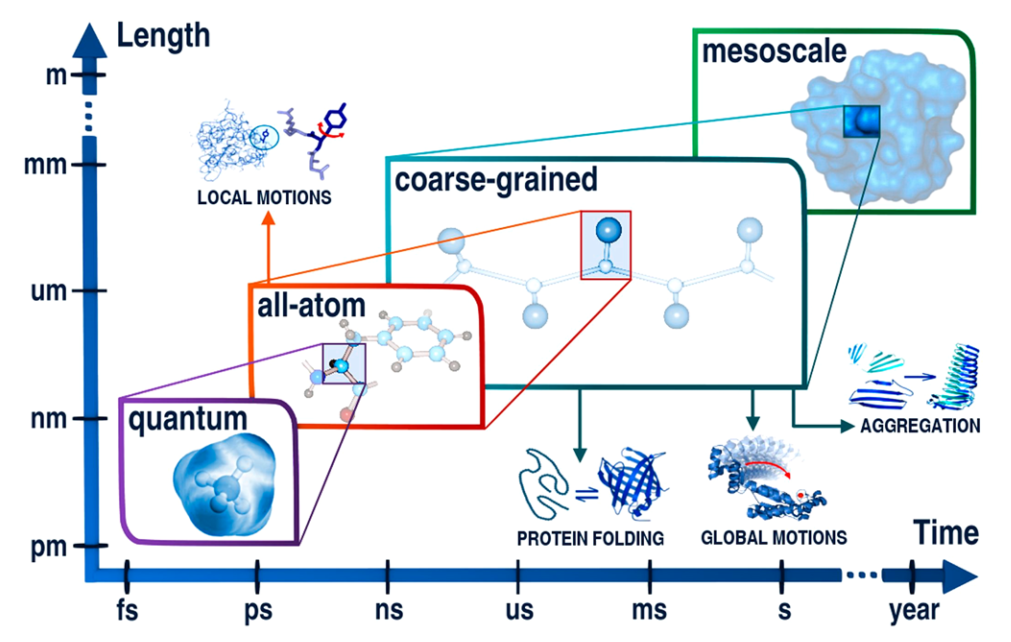
\includegraphics[width=0.7\linewidth]{scale}
	\caption{Different scales of common computational biology experiments \cite{Kmiecik2016}.}
	\label{fig:scale}
\end{figure}

The main objective of a coarse-grained representation is to reduce the number of degrees of freedom, replacing amino acids (either fragments or entire side chains) with pseudo-atoms. The first coarse-grained protein models were built in the 70's and were successfully able to simulate an entire folding process \cite{Levitt1975}. This early model consisted of pseudo atoms placed at $C\alpha$ positions and at the geometric center of protein side chains (except for glycine) and the only degree of freedom considered was the rotation angle along the central pseudo bond for three consecutive $C\alpha$ pseudo atoms. Interaction between united atoms was described as a simple Lennard-Jones potential.

Further development of the model accounted for the variable orientation of the pseudo sidechains and torsional potential for the main chain degrees of freedom were based on the statistical analysis of conformational properties of dipeptides \cite{Levitt1976}. Similar models aimed to represent residue-residue interactions using statistical potentials and Monte Carlo to simulate the folding process \cite{Wilson1989}.

Most proteins adopt a well-defined three-dimensional arrangement defined by both the conformational restraints of the main-chain as well as interactions with the environment by the side chains, characterizing a convoluted interplay of intra and intermolecular bonds that defines its structure. Henceforth, it is expected that a coarse-grained representation of a protein contains all its crucial elements. The main objective of this representation is to reduce the number of degrees of freedom inherent to a protein structure. 

The SICHO (side chain only) model considers only a pseudoatom placed in the center of each side chain, discarding backbone information; connectivity between pseudo atoms are given by statistically derived parameters observed in known structures \cite{Kolinski1998}. Novel methods such as The UNRES (united residue) \cite{Liwo2014} and CABS (C-alpha, beta and side chain) \cite{Kurcinski2015} included information about protein’s main chain as well as side chain. The Rosetta representation considers all backbone atoms and replaces the sidechain with a single pseudoatom \cite{johnson2004numerical} (Figure \ref{fig:rep}).

\begin{figure}
	\centering
	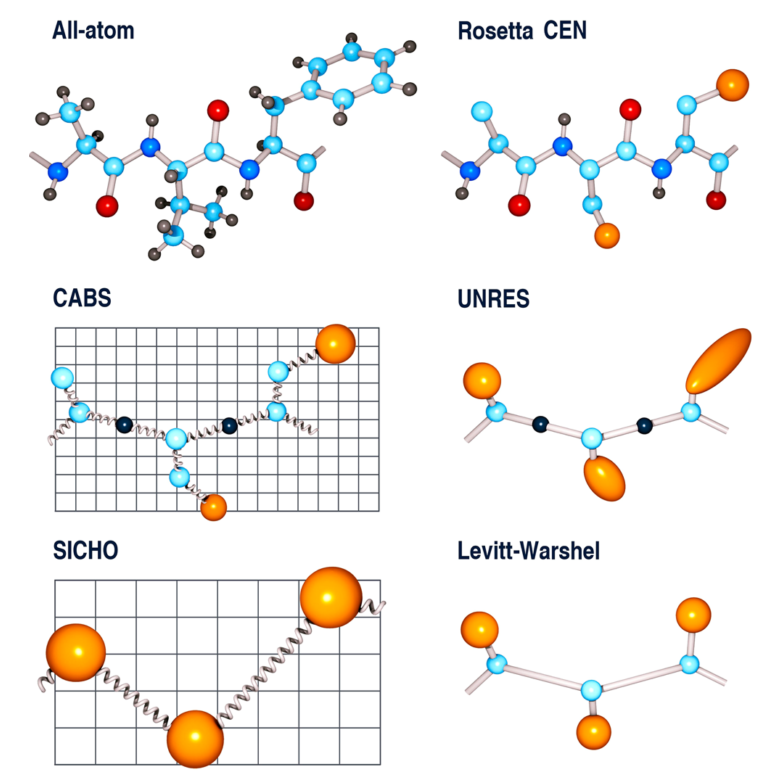
\includegraphics[width=0.7\linewidth]{rep}
	\caption{Different coarse-grained representations of a protein; united side chain atoms are colored in orange. pseudobonds of fluctuating length are shown as springs and lattice models are shown on the underlying lattice slide \cite{Kmiecik2016}.}
	\label{fig:rep}
\end{figure}

The balance between enthalpy and entropy are affected by the reduction of the system’s degrees of freedom. Since the impact in entropy is compensated by reducing the enthalpic terms, a coarse-grained model may accurately reproduce differences in free energy even though its enthalpy and entropy estimations might be inaccurate.

In order to develop coarse-grained force fields, efforts have been applied in two fronts; physics-based, following the same philosophy of it full-atom counterpart, basing it on molecular physics and knowledge-based that takes advantage the growing databases via statistical analysis. Here we will expound on the former, specifically on the MARTINI \cite{Marrink2007} force field.

\section{MARTINI Force Field}

The MARTINI force field was developed taking into heavy consideration the atomistic models, especially for bonded interactions. It aims for a broader range of applications instead of focusing on accurate reproductions of structural details at a specific point in a given system. For that purpose, the non-bonded interactions of chemical building blocks are extensively calibrated against experimental data. The main focus of this coarse-graining approach is to offer a computationally optimized and user-friendly model that is applicable to a wide range of biologically relevant systems.

This model is based on a four-to-one mapping, four heavy atoms (and associated hydrogens) are represented by a single atom (CG bead). Four real water molecules are represented as a single CG bead whilst ion CG bead representation takes into account both the ion and its hydration shell \cite{Marrink2013} (Figure \ref{fig:martini4to1}). The MARTINI model offers the following types of particles: charged (Q), apolar (C), non-polar (N) and polar (P); this is further expanded according to its hydrogen-bonding capabilities (donor, acceptor, both or none) or its degree of polarity ($1-5$) giving a total of 18 types of particles.

\begin{figure}
	\centering
	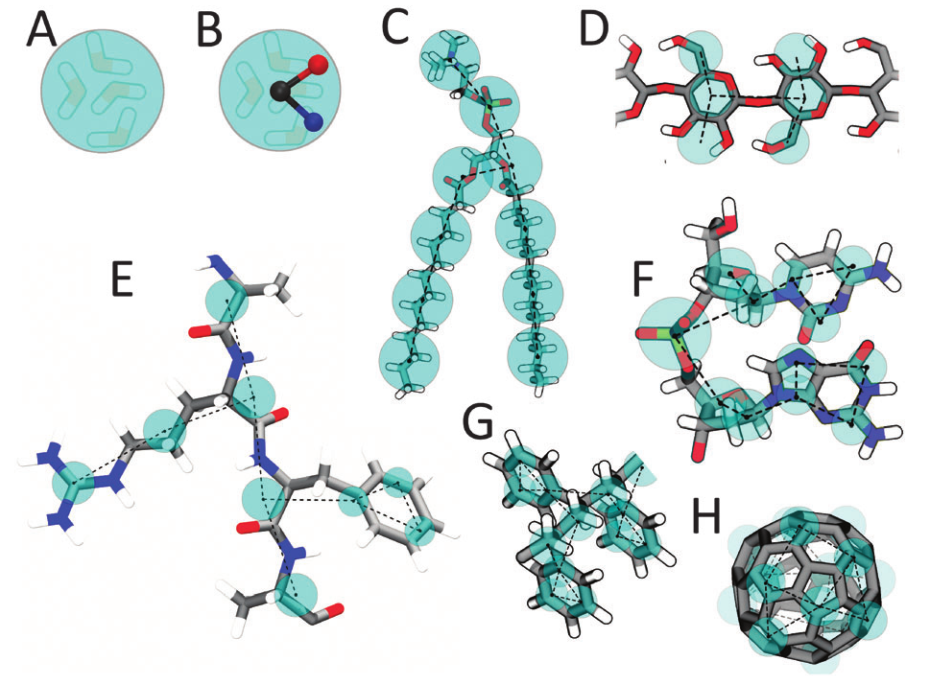
\includegraphics[width=0.7\linewidth]{martini_4to1}
	\caption{Examples of Martini mapping selected molecules. (A) Standard water particle. (B) Polarizable water molecule with embedded charges. (C) DMPC lipid. (D) Polysaccharide fragment. (E) Peptide. (F) DNA fragment. (G) Polystyrene fragment. (H) Fullerene molecule. In all cases Martini CG beads are shown as cyan transparent beads overlaying the atomistic structure \cite{Marrink2013}.}
	\label{fig:martini4to1}
\end{figure}

\textbf{Non-bonded} interactions are described by a Lennard-Jones (LJ) 12-6 potential (equation \ref{eq:01}), in which $\sigma_{ij}$ represents the closest distance of approach between particles $i, j$ and $\epsilon_{ij}$, the strength of the interaction. Effective particle size is defined as $\sigma=0.47nm$, if the given interaction is between charged (Q-type) and apolar (C-type) then $\sigma = 0.62nm$. This change in $\sigma$ favours Q-type particles to keep their hydration shell when placed into an apolar medium \cite{Marrink2007}.

\begin{equation}
E_{i,j}(r) = 4\epsilon \left [\left ( \frac{\sigma_{ij} }{r} \right )^{12} - \left ( \frac{\sigma_{ij} }{r} \right )^{6} \right ]
\label{eq:01}
\end{equation}

Charged groups have a full charge $q_{ij}$ that interacts via a Coulombic potential energy function (equation \ref{eq:02}), with dielectric constant for explicit screening.

% equation
\begin{equation}
U_{el}(r) = \frac{q_{i} q_{j}}{4\pi \epsilon_{0} \epsilon_{1} r}
\label{eq:02}
\end{equation}

Bonded interactions are described by a weak harmonic potential $V_{bond}(R)$

\begin{equation}
V_{bond}(R) = \frac{1}{2} K_{bond} \left ( R- R_{bond} \right )^2
\label{eq:03}
\end{equation}


with equilibrium distance $R_{bond} = 0.47 nm$ and a force constant of $K_{bond} = 1250 kJ mol^{-1} nm^{-2}$. To better represent the chemical structure of bonded interactions a weak harmonic potential $V_{angle}(\theta)$ is used 

\begin{equation}
V_{angle}(\theta ) = \frac{1}{2}K_{angle}\left \{ cos(\theta) -cos(\theta_{0}) \right \}^2
\label{eq:03}
\end{equation}

LJ interaction is not accounted for bonded particles but are calculated for second nearest neighbours \cite{Marrink2007}.

\section{MARTINI DNA Extension}

The MARTINI CG DNA model was systematically parametrized according to the MARTINI philosophy, being backwards compatible with all other MARTINI model implementations. Experimental values such as liquid densities and partitioning free energies of small solutes between polar and nonpolar solvents are used to determine non-bonded interaction parameters\cite{Uusitalo2015}.

As previously described, four non-hydrogen atoms are mapped to one CG bead which describes one or more chemical building blocks along with its properties. The parametrization used by Uusitalo and collaborators combines top-down (experimental data) and bottom-up (atomistic simulations) methodologies to parametrize the CG DNA model. The CG bead types for each nucleobase were selected based on partition free energies from water to chloroform or hydrated octanol. Bonded interactions have been fitted to reproduce dihedral, angle and bond distributions from atomistic simulation of short single stranded DNAs (ssDNAs). For double stranded DNA (dsDNA) an elastic network was devised to maintain the double helical structure.
	
Here each nucleotide is mapped to six or seven CG beads. The phosphate accounts for one bead and sugar for two, pyrimidines are represented as three-bead rings and purines as four-bead rings (Figure \ref{fig:dnacg}). After changing the representation of dsDNA bases the resulting distance between them are 0.34 nm, which lead to issues in the CG model. To account for that, a smaller bead size was created for the CG DNA model with $\sigma = 0.32nm$ (68\% smaller than the regular CG bead) and named T, for tiny. 

\begin{figure}
	\centering
	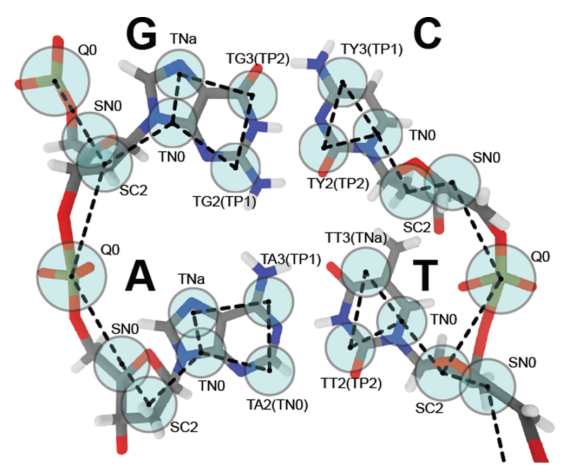
\includegraphics[width=0.7\linewidth]{dna_cg}
	\caption{DNA backbone is modeled with one bead describing the phosphate and two beads describing the sugar. The pyrimidines are modeled with three beads and the purines with four beads. T-prefix marks the beads that use the new tiny bead type. For hydrogen bonding beads, the new special bead types are shown together with the bead type describing their interactions with all beads except the special hydrogen bonding beads (in parentheses) \cite{Uusitalo2015}.}
	\label{fig:dnacg}
\end{figure}

Hydrogen bonding between bases is a crucial factor for the formation of dsDNA and since the standard MARTINI model does not describe the directional hydrogen bonds, the interaction between hydrogen bonding beads was tweaked. Interactions are defined in a pairwise fashion for each bead type, henceforth eight special beads were added for the purpose of replicating this crucial bond. 

\section{Integrative modelling of biomolecular complexes with HADDOCK}

Knowledge of the atomistic, three-dimensional, interaction between macromolecules is fundamental for the understanding of biological functions of organisms, provided by its three-dimensional structure. These structures may be obtained using experimental methods such as X-Ray crystallography, nuclear magnetic resonance (NMR) or cryo electron microscopy (Cryo-EM). The RCSB Protein Data Bank \cite{Berman2000} is the global repository for macromolecular structures with 125309 deposited structures (December/2016). Much can be studied and derived from experimentally solved complexes but the experimental obtention of three-dimensional complexes remain a timely, low throughput process.

Computational docking is a powerful tool to model three-dimensional structures of protein-protein, protein-DNA, protein-RNA and protein-small molecule interactions. By sampling a large number of possible conformations and selecting those with low interaction energies it is possible to obtain a native-like conformational of a macromolecular complex.

The high ambiguity driven docking approach software HADDOCK developed in Alexandre Bonvin Lab uses biochemical and/or biophysical interactions to predict macromolecular interactions and is renowned for its functionality and quality. Information on interacting residues was introduced as Ambiguous Interaction Restraints (AIRs) as means to drive the docking \cite{Dominguez2003}.

A worldwide experiment, the Critical Assessment of PRedicted Interactions (CAPRI) \cite{Janin2002} aims to evaluate the predictive power of docking software. HADDOCK was ranked in 2015 as the top software both in the Scorer and Server ranking categories \cite{HADDOCKCAPRI}.

\subsection{Docking protocol}

The docking approach is composed of python scripts derived from a software protocol called ARIA (Ambiguous Restraints for Iterative Assignment) \cite{Linge2001} used to integrate data from NRM into structure calculations and uses the highly flexible CNS (Crystallography \& NMR System) \cite{Brunger2013} software suit. Inter and intramolecular energies are accounted for using full electrostatic and van der Waals energy using the OPLS \cite{Jorgensen1988} nonbonded parameters and further optimizations. 

The docking protocol is executed in three steps: (1) rigid body energy minimizations after orientation randomization, \textit{it0}; (2) semirigid simulated annealing in torsion angle space, \textit{it1}; and (3) final refinement in Cartesian space with explicit solvent, \textit{water}.

In the first step (\textit{it0}), after two partner proteins are positioned at $150 \AA$ apart, each one is randomly rotated around its center of mass then submitted to a rigid body energy minimization. Firstly, four cycles of orientational optimization are executed so that each protein is allowed to rotate to minimize the intermolecular energy function, then macromolecules are allowed to both rotate and translate, thus performing the rigid body EM docking. 

During the second stage (\textit{it1}) there are three rounds of simulated annealing refinements; in the first one the two partners are considered rigid bodies and their orientation is optimized, in the second round the side chains at the interface are allowed to move and in the last both side chains and backbone (at the interface) are allowed to move in order to obtain the final conformational rearrangement.

On the last step of the docking protocol (\textit{water}), the interacting system is placed in a $8\AA$ shell of TIP3 water molecules \cite{Mark2001}, the system is heated to 300K with position restrains on all atoms except side chains. A short molecular dynamics is performed on the non-interface heavy atoms. On the final cooling stage the position restrains are limited to backbone atoms outside the interface.
Final structures are then clustered using pairwise backbone interface root mean square deviation with ($cutoff > 1.0 \AA$) and analyzed according to their average interaction energies $E_{elec}$, $E_{vdw}$ and $E_{acs}$ plus the average buried surface area. 

\chapter{Justification}

Alexandre Bonvin’s Lab is the Computational Structural Biology group at Utrecht University, located in the Netherlands. With high impact publications dating back to 1990, this research group is placed amongst the top ranking predictors and scorers on CAPRI. The use of experimental data to drive and/or validate its macromolecular predictions is one of the core methodologies used by this group and it yields exceptional results.

The proposed research project aims to implement and benchmark a coarse-grained DNA/RNA model into HADDOCK. The use of coarse-grained models has enabled researchers to simulate large-scale biomolecular processes on time scales that were previously inaccessible to full-atom models \cite{Inglfsson2013}. Its usefulness has been proved on the fields of protein folding \cite{Liwo1997}, mechanosensitive channels \cite{Louhivuori2010}, membrane protein self-assembly \cite{Periole2007} , DNA hybridization \cite{Sambriski2009} amongst many others. 

This implementation will build upon a previous successful and thoroughly optimized implementation of the MARTINI Protein-Protein CG force field in HADDOCK (unpublished) and will facilitate computational biology studies with proteins and nucleic acids to accompany the ever growing scale and resolution of structural data.

As an example, the yeast RNA polymerase III elongation complex was determined at $3.9\AA$ using Cryo-EM \cite{Hoffmann2015} consisting of 39284 atoms (without water), large systems such as this and the nucleossome with fibers varying from 10-nm to 30-nm \cite{Silva2015}, are the most adequate targets for CG models, granting deeper understanding of such relevant systems.

For such, a capable implementation done according to both the MARTINI philosophy and taking advantage HADDOCK’s integrative approach to macromolecular interactions and its lab members competences, followed by a thorough benchmarking will lay the groundwork for profound studies of large scale macromolecular processes.	

\chapter{Objectives}
\section{General}
Develop and implement a coarse-grained DNA/RNA model in HADDOCK and benchmark it for docking.
\section{Specific}

\begin{itemize}
	\item Convert MARTINI coarse-grained DNA/RNA topology into CNS format (Crystallography \& NMR System)
	\item Add and test forcefield in HADDOCK
	\item Convert Protein-DNA/RNA dataset do CG
	\item Run docking trials
	\item Evaluate results
	\item Optimize scoring functions
	\item Implement CG Protein-DNA/RNA docking
\end{itemize}

%\begin{landscape}
\chapter{Workplan}

The first month will be dedicated to setup, convert and initiate the CG force field testing. During the second month the testing phase will be completed and we proceed to the first docking trials and result evaluation, this stage will be executed iteratively with the scoring function optimization. Optimization will be concluded on the last month and the CG Protein-DNA/RNA docking routine will be implemented followed by the redaction of a report and the research article (Table \ref{table:workplan}).
\\
\\
\\

% Please add the following required packages to your document preamble:
% \usepackage[table,xcdraw]{xcolor}
% If you use beamer only pass "xcolor=table" option, i.e. \documentclass[xcolor=table]{beamer}
\begin{table}[h]
	\centering
	\caption{Proposed workplan}
	\label{table:workplan}
	\begin{tabular}{|L{5cm}|c|c|c|c|c|c|}
		\hline
		& \multicolumn{1}{l|}{Month 1} & \multicolumn{1}{l|}{Month 2} & \multicolumn{1}{l|}{Month 3} & \multicolumn{1}{l|}{Month 4} & \multicolumn{1}{l|}{Month 5} & \multicolumn{1}{l|}{Month 6} \\ \hline
		\rowcolor[HTML]{EFEFEF} 
		Convert CG topology into CNS format   & \textbf{X}                   & \textbf{}                    & \textbf{}                    & \textbf{}                    & \textbf{}                    & \textbf{}                    \\ \hline
		Convert Protein-DNA/RNA dataset to CG & \textbf{X}                   & \textbf{}                    & \textbf{}                    & \textbf{}                    & \textbf{}                    & \textbf{}                    \\ \hline
		\rowcolor[HTML]{EFEFEF} 
		Add and test forcefield in HADDOCK    & \textbf{}                    & \textbf{X}                   & \textbf{}                    & \textbf{}                    & \textbf{}                    & \textbf{}                    \\ \hline
		Run docking trials                    & \textbf{}                    & \textbf{X}                   & \textbf{}                    & \textbf{}                    & \textbf{}                    & \textbf{}                    \\ \hline
		\rowcolor[HTML]{EFEFEF} 
		Evaluate results                      & \textbf{}                    & \textbf{}                    & \textbf{X}                   & \textbf{}                    & \textbf{}                    & \textbf{}                    \\ \hline
		Optimize scoring functions            & \textbf{}                    & \textbf{}                    & \textbf{X}                   & \textbf{X}                   & \textbf{}                    & \textbf{}                    \\ \hline
		\rowcolor[HTML]{EFEFEF} 
		Implement CG Protein-DNA/RNA docking  & \textbf{}                    & \textbf{}                    & \textbf{}                    & \textbf{X}                   & \textbf{X}                   & \textbf{}                    \\ \hline
		Write report and research article     & \textbf{}                    & \textbf{}                    & \textbf{}                    & \textbf{}                    & \textbf{X}                   & \textbf{X}                   \\ \hline
	\end{tabular}
\end{table}

%\begin{table}[h]
%	\centering
%	\caption{Proposed workplan}
%	\label{table:workplan}
%	\begin{tabular}{|L{6cm}|c|c|c|}
%		\hline
%		\rowcolor[HTML]{C0C0C0} 
%		& \multicolumn{1}{l|}{\cellcolor[HTML]{C0C0C0}September/2017} & \multicolumn{1}{l|}{\cellcolor[HTML]{C0C0C0}October/2017} & \multicolumn{1}{l|}{\cellcolor[HTML]{C0C0C0}November/2017} \\ \hline
%		Convert CG topology into CNS format   & \textbf{X}                                                  & \textbf{}                                                 & \textbf{}                                                  \\ \hline
%		\rowcolor[HTML]{EFEFEF} 
%		Convert Protein-DNA/RNA dataset do CG & \textbf{X}                                                  & \textbf{}                                                 & \textbf{}                                                  \\ \hline
%		Add and test forcefield to HADDOCK    & \textbf{X}                                                  & \textbf{X}                                                & \textbf{}                                                  \\ \hline
%		\rowcolor[HTML]{EFEFEF} 
%		Run docking trials                    & \textbf{}                                                   & \textbf{X}                                                & \textbf{}                                                  \\ \hline
%		Evaluate results                      & \textbf{}                                                   & \textbf{X}                                                & \textbf{X}                                                 \\ \hline
%		\rowcolor[HTML]{EFEFEF} 
%		Optimize scoring functions            & \textbf{}                                                   & \textbf{X}                                                & \textbf{X}                                                 \\ \hline
%		Implement CG Protein-DNA/RNA docking  & \textbf{}                                                   & \textbf{}                                                 & \textbf{X}                                                 \\ \hline
%		\rowcolor[HTML]{EFEFEF} 
%		Write report and research article     & \textbf{}                                                   & \textbf{}                                                 & \textbf{X}                                                 \\ \hline
%	\end{tabular}
%\end{table}


%\end{landscape}
% insert table

\chapter{Methods ans Result Analysis}


The overview workflow of the proposed methods is presented in Figure \ref{fig:flow}.

\begin{figure}[h]
	\centering
	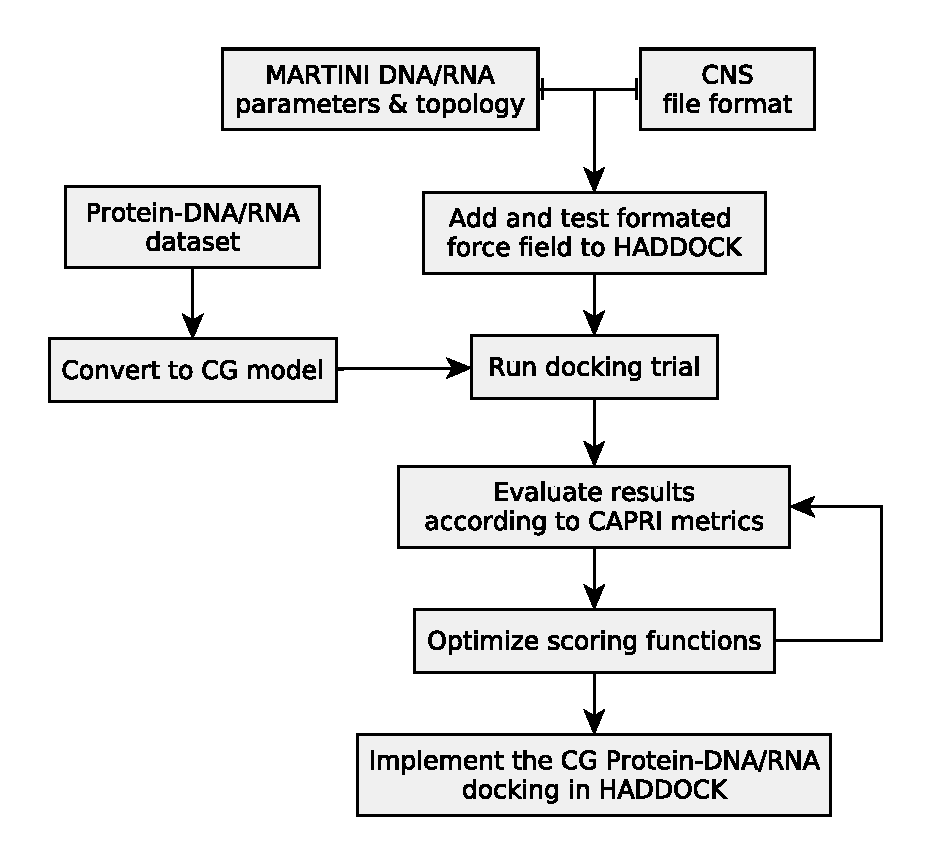
\includegraphics[width=0.7\linewidth]{flow}
	\caption{Overview of the proposed implementation.}
	\label{fig:flow}
\end{figure}

\section{All-atoms to CG conversion}

The conversion of the structures to CG models will be carried out by a conversion script adapted from the one provided by the research group responsible for MARTINI. It will be adapted to output distance restraints between the atoms mapped to one CG particle and the other CG particle. These distance restraints are use in an original procedure in HADDOCK to map back the CG model to an all-atom models, while allowing for conformational changes.

\section{Topology and parameter conversion}

The first step of the implementation is to convert the MARTINI DNA/RNA topology and parameters to the CNS format used by HADDOCK. The topology is consisted of information such as, description of atoms, assignment of covalent bonds, bond angles, charge and others that are combined in order to form the macromolecule. The parameters correspond to force constants and equilibrium values for the various energy terms.

\begin{figure}
	\centering
	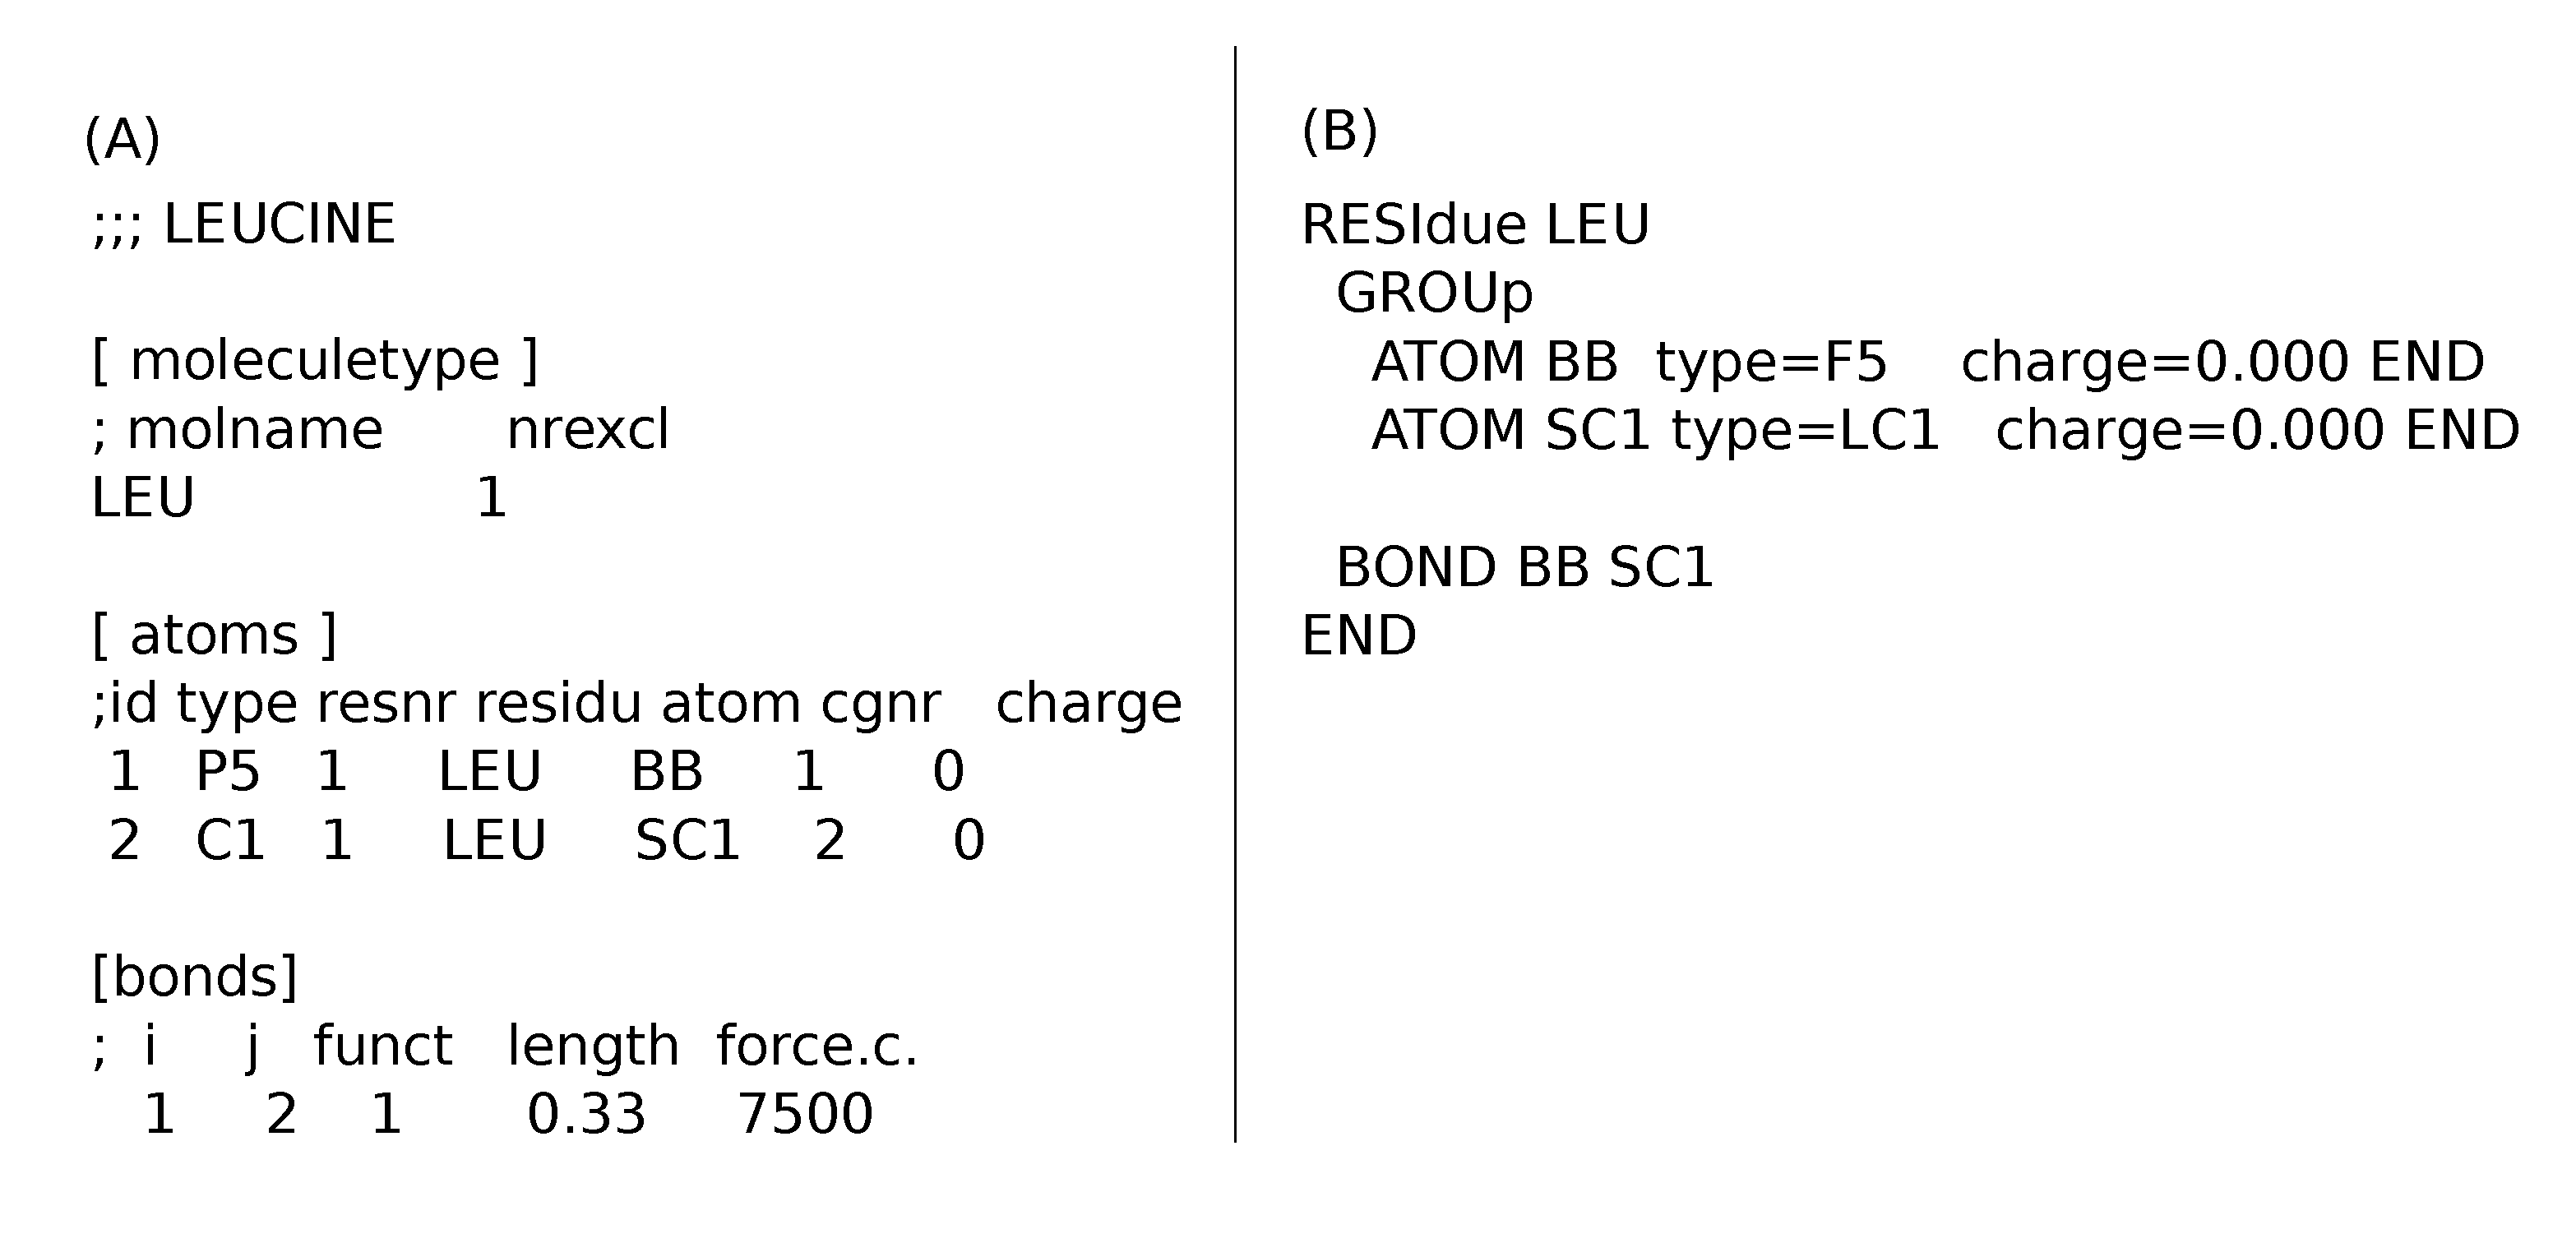
\includegraphics[width=0.7\linewidth]{file_formats}
	\caption{Example of MARTINI (A) and CNS (B) topology for the amino acid leucine.}
	\label{fig:fileformats}
\end{figure}

\section{Docking trials}

After integration of the MARTINI CG DNA/RNA force field into HADDOCK, its performance will be evaluated using a benchmark of Protein-DNA complexes \cite{vanDijk2008}. The benchmark (v1.3) is comprised of 47 test cases divided into classes of cases; easy (13), intermediate (22) and difficult (12). Its difficulty is set according to the degree of structural rearrangement after complex formation. Most of DNA binding protein types are covered according to the Luscombe classification \cite{Luscombe2000}.

Docking will be performed using the same information about interfaces as used in the original benchmark. For this, 	sxperimental or computational data about the interaction interface can be provided to generate \textit{Ambiguous Interaction Restraints} (AIRs) between potential interacting residues \cite{Dominguez2003}. These AIRs are responsible for directing the docking process by defining active residues, potentially involved or passive residues, the solvent-accessible neighbours of the active residues.  AIRs are defined for all active residues by calculating its effective distances, $d^{eff}$ as follows:

\begin{equation}
d_{iAB}^{eff} =  \left ( \sum_{M_{iA}=1}^{N_{res}B} \sum_{K=1}^{N_{atoms}} \sum_{N_{kB}=1}^{N_{atoms}} \frac{1}{d_{m_{iA\; n\; kB}}^{6}} \right ) ^ \frac{-1}{6}
\label{eq:04}
\end{equation}

Where $N_{atoms}$ represents all atoms of a certain residue in both units of the interacting complex, $N_{resB}$ is the sum of active and passive residues, $i$ is the interaction of all restrains; the $\frac{-1}{6}$ sum reassembles the Lennard-jones potential. 

\section{Result evaluation}

The generated docking solutions will be assessed based on CAPRI \cite{Janin2002} criteria, measuring two root mean square deviations (RMSD) calculated over the backbone atoms. Resulting complexes will be categorized into Incorrect, Acceptable, Medium and High according to their interface RMSD (i-RMSD) and ligand RMSD (l-RMSD) (Table \ref{table:capri-table}). 

% Please add the following required packages to your document preamble:
% 
% If you use beamer only pass "xcolor=table" option, i.e. \documentclass[xcolor=table]{beamer}
\begin{table}[h]
	\centering
	\caption{CAPRI categorization of macromoecular complexes}
	\label{table:capri-table}
	\begin{tabular}{|c|c|}
		\hline
		\rowcolor[HTML]{C0C0C0} 
		Category   & RMSD \AA                          \\ \hline
		Incorrect  & i-RMSD $\geq$ 4.0 or l-RMSD $\geq$ 10.0 \\ \hline
		Acceptable & i-RMSD $\leq$ 4.0 or l-RMSD $\leq$ 10.0 \\ \hline
		Medium     & i-RMSD $\leq$ 2.0 or l-RMSD $\leq$ 5.0  \\ \hline
		High       & i-RMSD $\leq$ 1.0 or l-RMSD $\leq$ 1.0  \\ \hline
	\end{tabular}
\end{table}

\section{DNA/RNA scoring function optimization}

Each step of the HADDOCK’s docking protocol; \textit{Rigid body}, \textit{Flexible} and \textit{Refinement}, has its own scoring function defined as the weighted sum of interaction energies and buried surface area (BSA):

\begin{equation}
\emph{Rigid body (it0)} = 0.01 E_{air} + 0.01 E_{vdw} + 1.0 E_{elec} + 1.0 E_{desolv} - 0.01 BSA
\label{eq:05}
\end{equation}

\begin{equation}
\emph{Flexible (it1)} = 0.01 E_{air} + 1.0 E_{vdw} + 1.0 E_{elec} + 1.0 E_{desolv} - 0.01 BSA
\label{eq:06}
\end{equation}

\begin{equation}
\emph{Refinement (water)} = 0.1 E_{air} + 1.0 E_{vdw} + 0.2 E_{elec} + 1.0 E_{desolv}
\label{eq:07}
\end{equation}

Optimization of the scoring functions will consist of an evaluation of different ranges of weights in each of interaction energies and comparison with the CAPRI evaluation in order to obtain optimal weights to correctly identify the best generated complexes (Figure \ref{fig:optimization}) and maximize the number of near-native models selected at the rigid-body docking stage. Final optimal weights are based on the average of optimal weight for each conformation for each complex in the benchmark.

Previous studies have shown that protein-DNA binding at the minor groove is driven by the large entropic release of ordered water despite unfavourable enthalpy. Nonetheless, this effect is not representative of a hydrophobic force since water ordering in the DNA is not determined by the apolar groups. This ordering is a consequence of the arrangement of polar groups to stabilize ice-like water organization in the groove \cite{Privalov2007}. Thus, it will be important to also check if desolvation effects can be neglected.

\begin{figure}
	\centering
	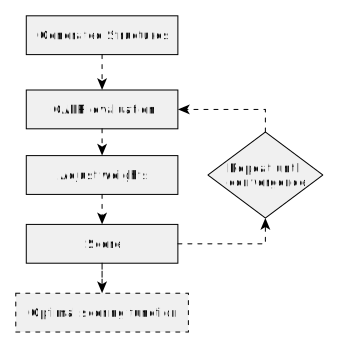
\includegraphics[width=0.7\linewidth]{optimization}
	\caption{Diagram of the score optimization}
	\label{fig:optimization}
\end{figure}


% ----------------------------------------------------------
% Capitulo com exemplos de comandos inseridos de arquivo externo 
% ----------------------------------------------------------

\include{abntex2-modelo-include-comandos}

% ---
% Finaliza a parte no bookmark do PDF
% para que se inicie o bookmark na raiz
% e adiciona espaço de parte no Sumário
% ---
\phantompart


% ----------------------------------------------------------
% ELEMENTOS PÓS-TEXTUAIS
% ----------------------------------------------------------
\postextual

% ----------------------------------------------------------
% Referências bibliográficas
% ----------------------------------------------------------
\bibliography{BonvinLab_RVH_2017}

% ----------------------------------------------------------
% Glossário
% ----------------------------------------------------------
%
% Consulte o manual da classe abntex2 para orientações sobre o glossário.
%
%\glossary

% ----------------------------------------------------------
% Apêndices
% ----------------------------------------------------------


%---------------------------------------------------------------------
% INDICE REMISSIVO
%---------------------------------------------------------------------

\phantompart

\printindex


\end{document}
